% !TEX root = MAIN.tex

\chapter{General Description}

\section{MASS}

\subsection{Product perspective}

% The IRD shall describe the product external interfaces to other systems

In this section, we provide a brief description of the external interfaces of the Mutation Analysis for Space Software (MASS) toolset.

Given that the objective of MASS is to assess test suites quality through mutation analysis, it means that the toolset mainly interacts with the SUT and its respective test suite. More specifically, MASS shall access the SUT source code, SUT test suite, and be able to run and collect information about test suite execution.

\subsection{Operational environment}

% Context diagrams may support this narrative description to summarize external interfaces and system block diagrams to show how the activity fits within the larger system.

\begin{figure}[t]
  \centering
  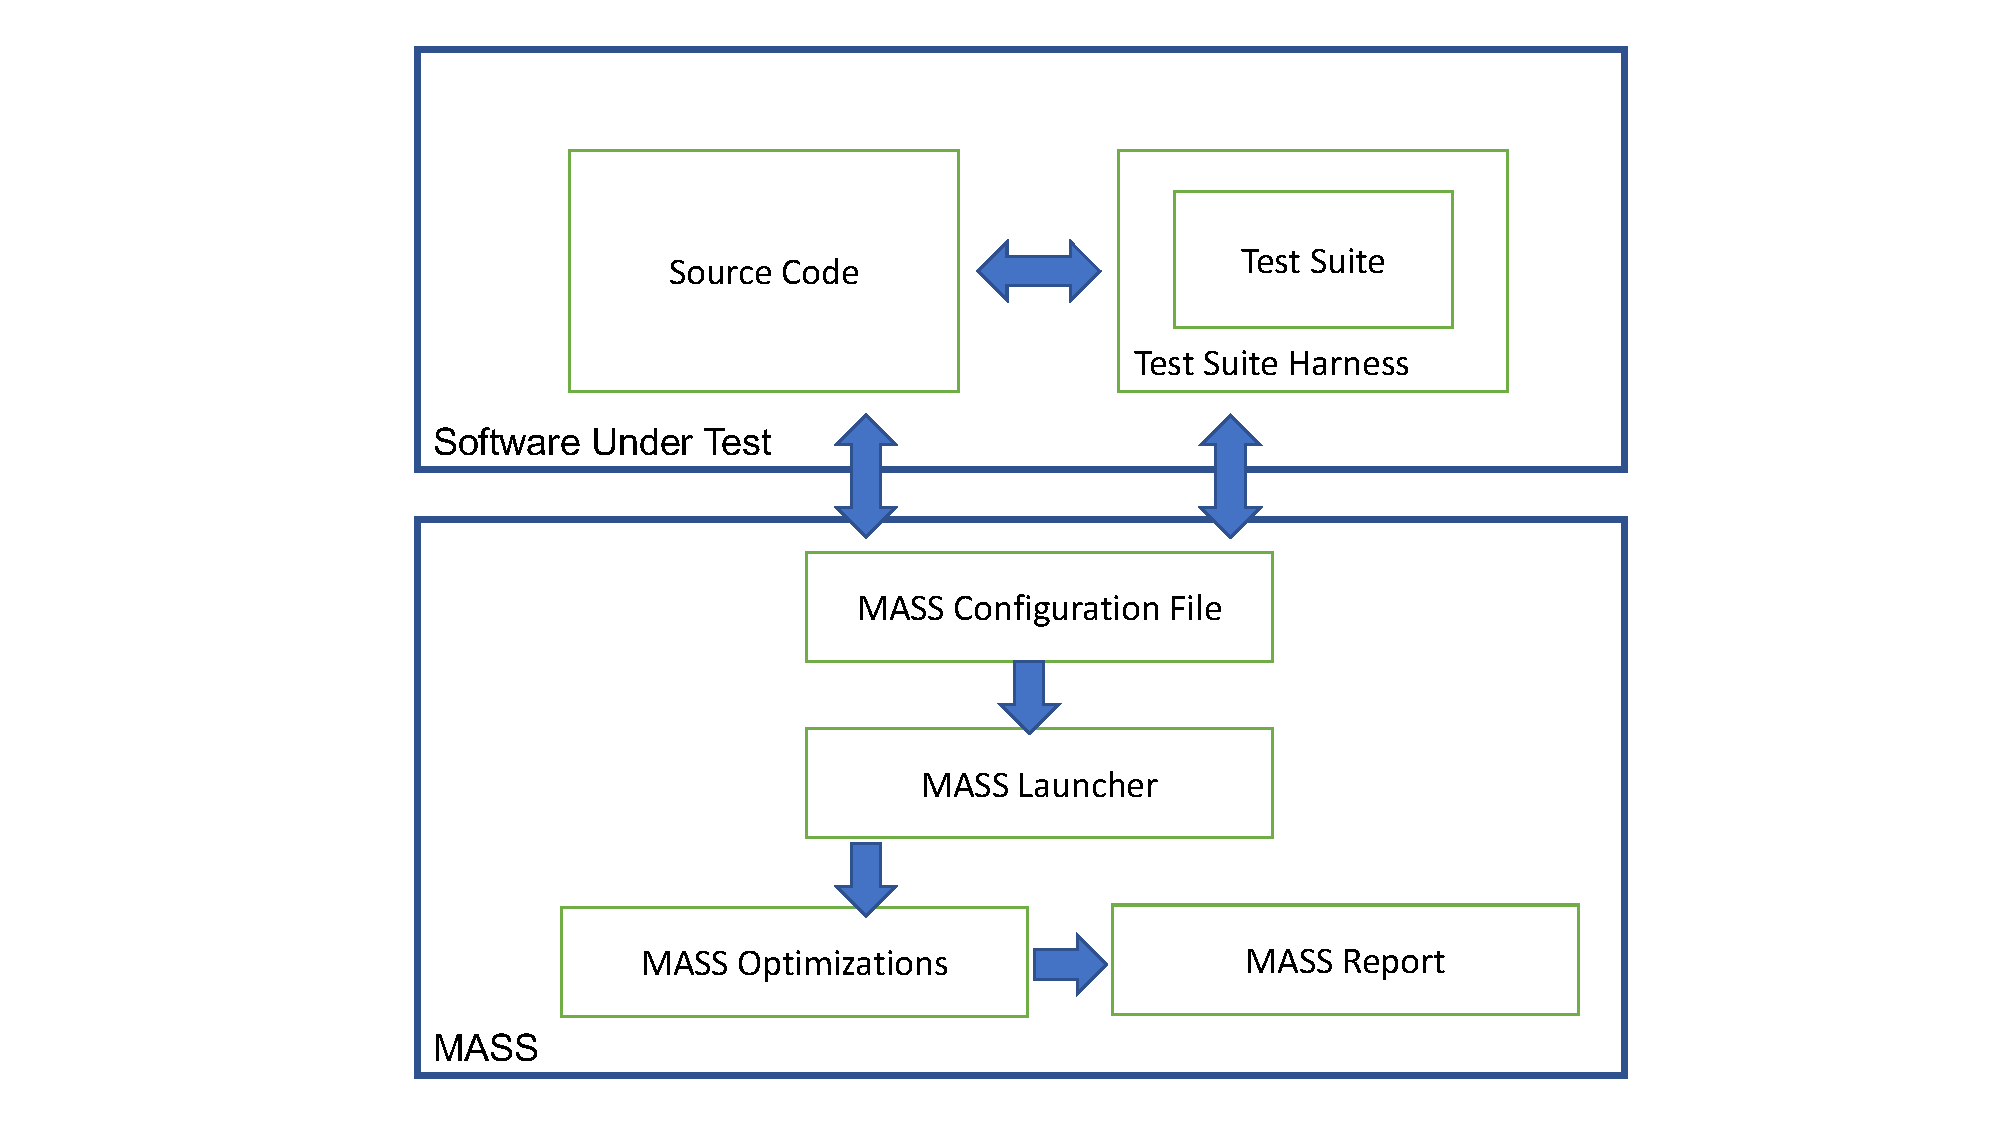
\includegraphics[width=0.7\textwidth]{images/mass-external.pdf}
      \caption{System block diagram of MASS' external interfaces.}
      \label{fig:mass:external}
\end{figure}

Figure~\ref{fig:mass:external} shows MASS' external interfaces through a system block diagram.
As shown in Figure~\ref{fig:mass:external}, MASS mainly interacts with the SUT through a configuration file, where engineers shall specify a set of Bash variables that enable MASS to correctly identify the SUT paths (e.g., source code folder, test suite folder), SUT compilation commands, the SUT test suite execution commands, and the configuration of MASS itself (e.g., trivial compiler optimizations flags, mutant selection strategy, sampling rate).


% \subsection{Assumption and dependencies}

\section{SEMuS}

\subsection{Product perspective}

In this section, we provide a brief description of the external interfaces of the Symbolic Execution-based Mutation Analysis Engine for Space Software (SEMuS).

SEMuS is an extension of SEMu, a symbolic execution engine based on KLEE, for this reason the product interacts mainly with the interfaces of KLEE-SEMu, and shall be properly configured for it. Additionally, the software interacts with the SUT, since it needs to parse the source code for test template generation, and also interacts with MASS, since the software needs to process the list of mutants for which inputs shall be generated.


\subsection{Operational environment}

\begin{figure}[t]
  \centering
  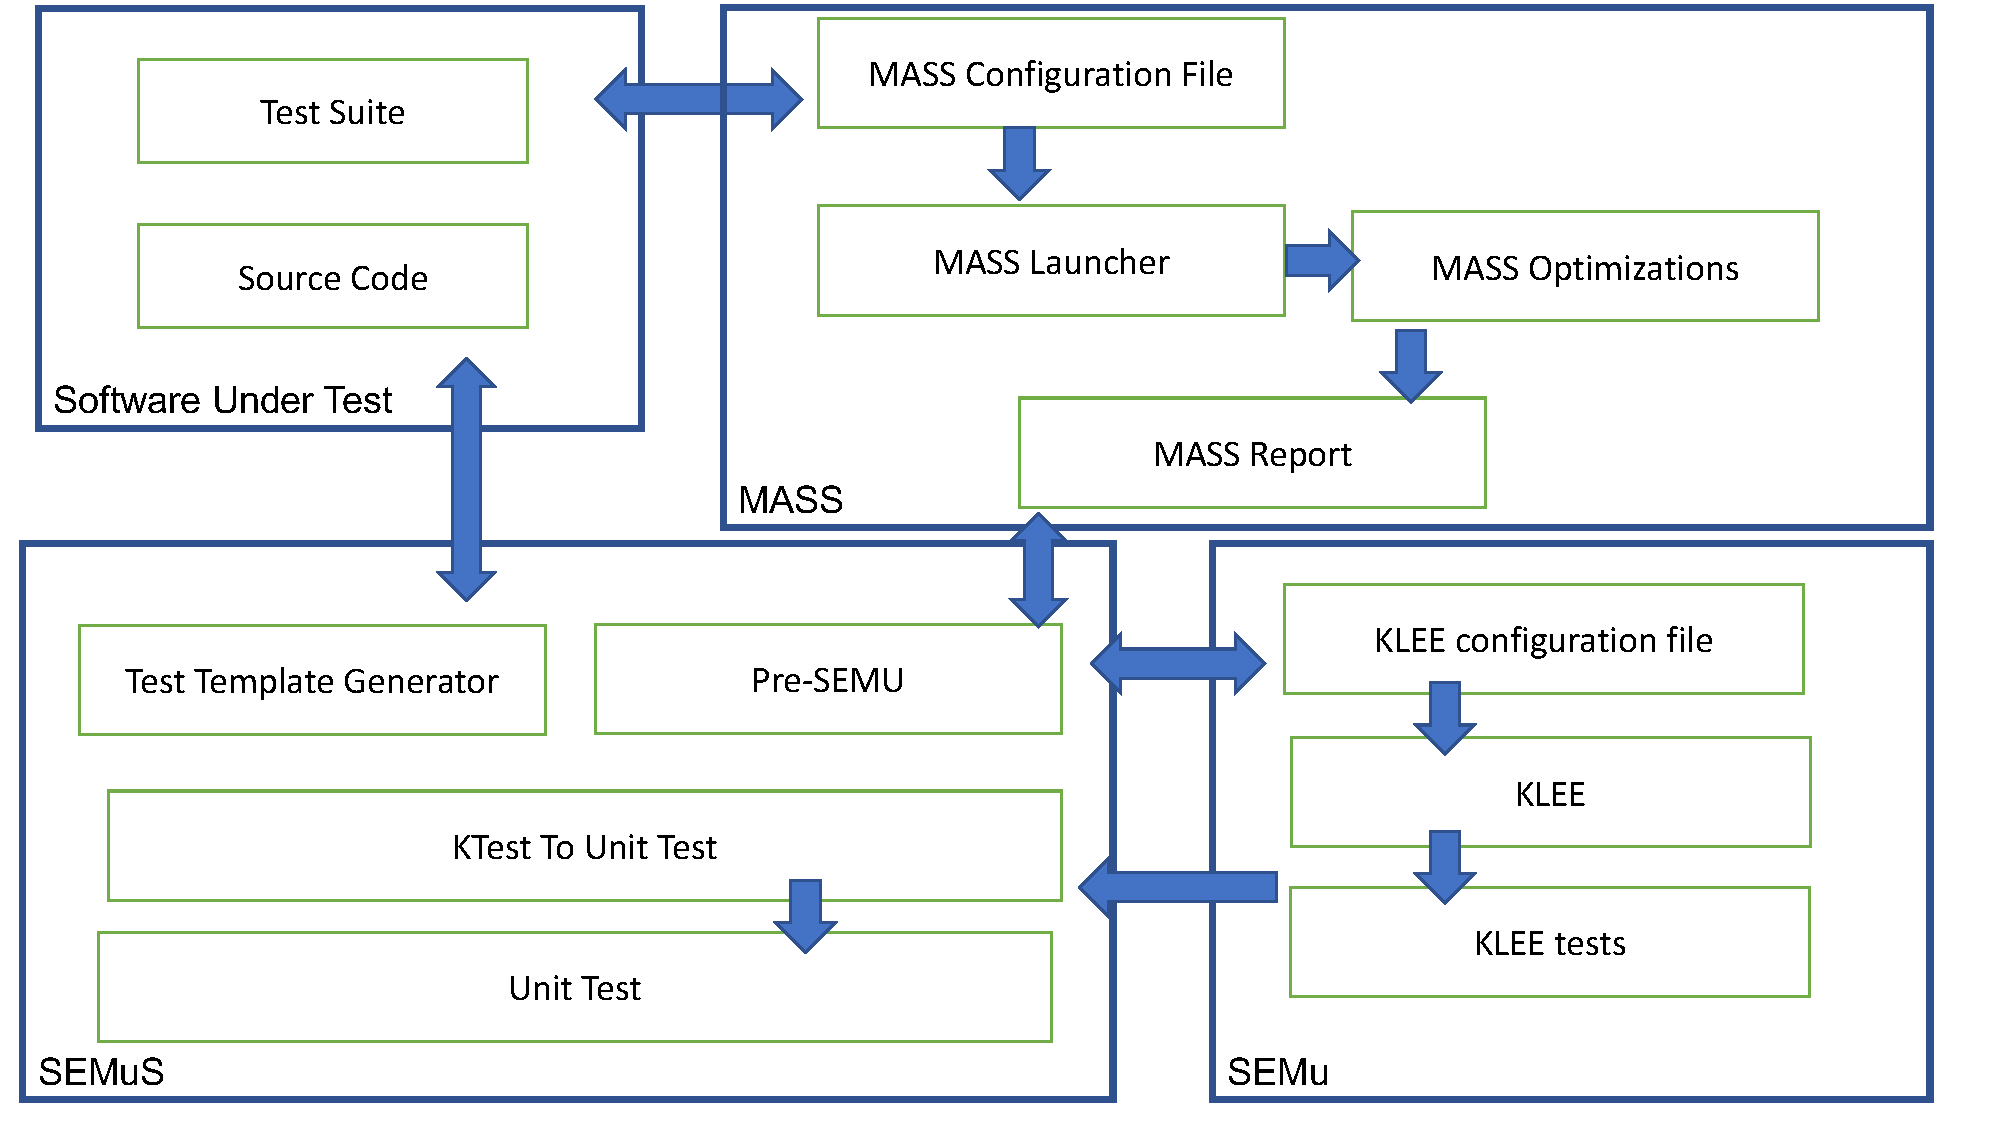
\includegraphics[width=0.7\textwidth]{images/semus-external.pdf}
      \caption{System block diagram of SEMuS' external interfaces.}
      \label{fig:semus:external}
\end{figure}

Figure~\ref{fig:semus:external} shows SEMuS' external interfaces through a system block diagram.
As shown in Figure~\ref{fig:semus:external}, SEMuS interacts with three external systems (1) the SUT, (2) the MASS toolset, and (3) the SEMu.

Firstly, SEMuS interacts with the SUT by means of a configuration file, where engineers shall specify a set of Bash variables that enable SEMuS to correctly identify the SUT paths (e.g., source code folder), SUT compilation commands, the configuration of SEMuS (e.g., output folder), and the configuration of SEMu (e.g., configuration of the heuristics, timeouts, maximum memory to be used).

Secondly, SEMuS interacts with MASS by means of the previously generated \emph{MASS report}, which provides information about the live and killed mutants. The information of live mutants is then used by SEMuS in order to generate test inputs only for the selected mutants.
The engineers shall setup the SEMuS configuration file to provide the path to the MASS report.

Lastly, SEMuS interacts with SEMu by means of the \emph{SEMu Wrapper}, a Python script that setups the KLEE configuration file and invokes SEMu. If test inputs are generated for the specified mutants, KLEE-SEMu will produce KLEE tests that shall be processed by the \emph{KTest To Unit Test} component.

\section{DAMAt}

\subsection{Product perspective}

% The IRD shall describe the product external interfaces to other systems

In this section, we provide a brief description of the external interfaces of the DAta-driven Mutation Analysis with tables (DAMAt) toolset.

Given that the objective of DAMAt is to assess the quality of test suites through data-driven mutation analysis, it means that the toolset mainly interacts with the SUT and its respective test suite. More specifically, DAMAt shall access the SUT source code, SUT test suite, and be able to run and collect information about test suite execution.

\subsection{Operational environment}

% Context diagrams may support this narrative description to summarize external interfaces and system block diagrams to show how the activity fits within the larger system.

\begin{figure}[t]
  \centering
  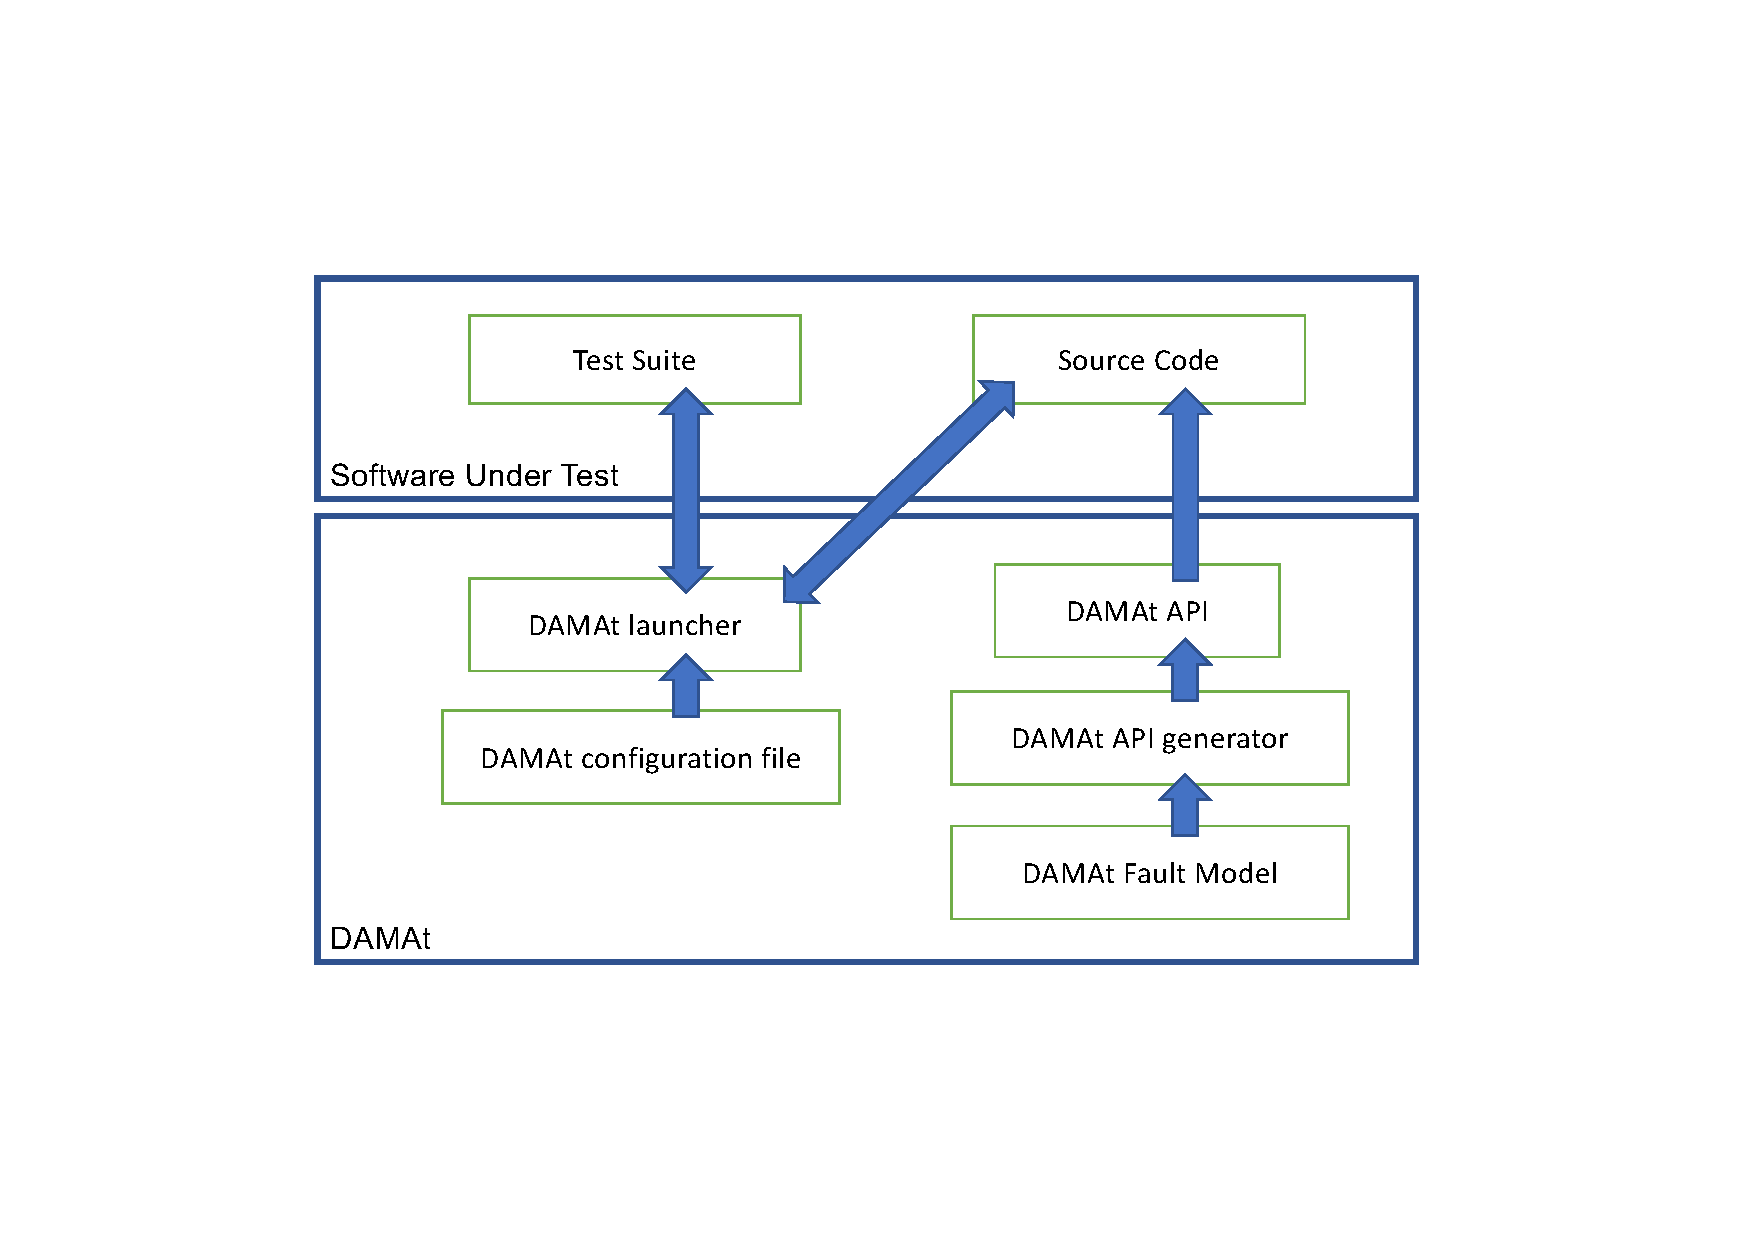
\includegraphics[width=0.7\textwidth]{images/damat-external.pdf}
      \caption{System block diagram of the external interfaces of DAMAt.}
      \label{fig:damat:external}
\end{figure}

Figure~\ref{fig:damat:external} shows DAMAt's external interfaces through a system block diagram.
As shown in Figure~\ref{fig:damat:external}, DAMAt interacts with the SUT through a launcher, that compiles the mutants, runs the test cases, and collects information about the executions and the results.

The correct paths (e.g source code folders ) and configuration variables (e.g. data type of the buffer targeted by the mutation) are set in the DAMAt configuration file by the user as bash variables.

DAMAt also interacts with the source code through calls to a mutation API containing the mutation logic. These calls shall be manually inserted by the user into the source code.
The mutation API is automatically generated starting from a fault model specified by the user.


% \subsection{Assumption and dependencies}
